\chapter{Реализация транзакций, обработка ошибок и динамический SQL}
\section{Управление транзакциями и параллелизм}

Транзакция — это логическая единица работы. Либо вся работа выполняется
как единое целое, либо она не выполняется вовсе.
В SQL Server все изменения данных в базе данных происходят в виде транзакций. 





\subsection{Свойства транзакций ACID}


\begin{itemize}
	\item \textbf{Атомарность} (atomicity). Каждая транзакция является атомарной единицей работы. Это означает, что в транзакции либо выполняются все изменения базы
	данных, либо ни одно из них. 
	\item \textbf{Согласованность} (consistency). Каждая транзакция, как завершившаяся, так и
	прерванная, оставляет базу данных в согласованном состоянии, как определяется всеми ограничениями объектов и базы данных. При возникновении несогласованного состояния SQL Server выполнит откат транзакции, чтобы поддержать
	согласованное состояние. 
	\item \textbf{Изоляция} (isolation). Каждая транзакция выполняется так, как будто она существует в изоляции от всех остальных транзакций по отношению к изменениям в
	базе данных. Степень изолированности может меняться в зависимоси от уровня
	изоляции. 
	\item  \textbf{Устойчивость} (durability). Каждая транзакция претерпевает прерывание сервиса. Когда сервис восстанавливается, все зафиксированные (committed) транзакции накатываются (зафиксированные изменения в базе данных завершены), а
	все нефиксированные транзакции откатываются (нефиксированные изменения
	удаляются). 
\end{itemize}

SQL Server поддерживает транзакционную устойчивость с помощью журнала транзакций базы данных. Любое изменение базы данных (инструкция модификации
данных или инструкция DDL) сначала записывается в журнал транзакций, с исходной версией данных (в случае обновлений и удалений). Когда транзакция зафиксирована и прошли все проверки согласованности, факт успешной фиксации транзакции записывается в журнал транзакций. 

\begin{figure}[h!]
	\begin{center}
		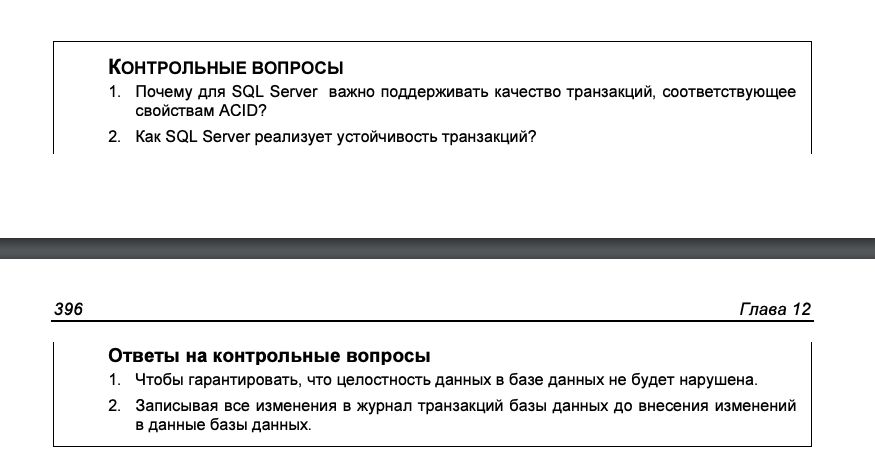
\includegraphics[width=0.6\textwidth]{img/control28.png}
	\end{center}
	\captionsetup{justification=centering}
\end{figure}


\subsection{Типы транзакций}

\begin{itemize}
	\item \textbf{Системные транзакции}. SQL Server использует системные транзакции для поддержки всех своих внутренних постоянных системных таблиц. Пользователи не могут управлять этими транзакциями. 
	\item \textbf{Пользовательские транзакции}. Транзакции, создаваемые пользователями в процессе изменения или даже чтения данных, либо автоматически, т. е. неявно, либо явно, называются пользовательскими транзакциями.
\end{itemize}

\subsection{Команды транзакций}

\begin{itemize}
	\item BEGIN TRANSACTION (BEGIN TRAN)
	\item COMMIT TRANSACTION (COMMIT TRAN) (COMMIT WORK) (COMMIT)
	\item ROLLBACK TRANSACTION (ROLLBACK)
\end{itemize}

\subsection{Уровни и состояния транзакций}

Уровень транзакции и ее состояние можно определить с помощью двух системных
функций. 

\begin{itemize}
	\item Функцию @@TRANCOUNT можно запросить для того, чтобы узнать уровень вложенности транзакции. Уровень, равный 0, указывает, что в данный момент код находится не внутри
	транзакции. Уровень больше 0 указывает, что транзакция активна, при этом если значение
	больше 1, то оно указывает уровень вложенности для вложенных транзакций. 
	\item Функцию XACT\_STATE() можно запросить для определения состояния транзакции.  Состояние, равное 0, указывает на то, что это неактивная транзакция. Состояние, равное 1, указывает, что это незафиксированная транзакция, которая может быть зафиксирована, но не известен уровень ее вложенности. Состояние, равное –1, указывает, что имеется незафиксированная транзакция,
	но она не может быть зафиксирована из-за предшествующей фатальной
	ошибки. 
\end{itemize}


\subsection{Режимы транзакций}

\begin{itemize}
	\item автофиксация (autocommit); 
	\item неявная транзакция (implicit transaction); 
	\item явная транзакция (explicit transaction). 
\end{itemize}


\subsection{Режим автоматической фиксации}
В режиме автоматической фиксации модификация данных и инструкции DDL языка T-SQL выполняются как транзакция, которая будет автоматически зафиксирована, если инструкция выполнена без ошибок, в противном случае будет выполнен
откат транзакции. Режим автоматической фиксации является режимом управления транзакциями по умолчанию.



В режиме автоматической фиксации не требуется никаких других команд управления транзакциями, таких как BEGIN TRAN, ROLLBACK TRAN или COMMIT TRAN. 

\subsection{Режим неявных транзакций}

В режиме неявных транзакций, когда выполняется одна или более инструкция DML или DDL либо инструкция SELECT, SQL Server запускает транзакцию, увеличивает @@TRANCOUNT, но не выполняет автоматической фиксации
или отката инструкции.

\begin{lstlisting}[label=lst:funcReturn, language=sql]
	SET IMPLICIT_TRANSACTIONS ON;
\end{lstlisting}


\begin{figure}[h!]
	\begin{center}
		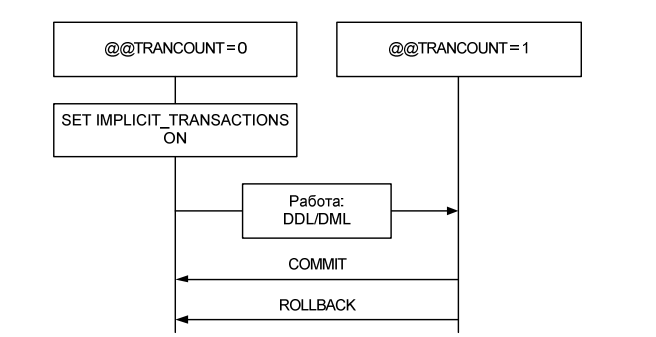
\includegraphics[width=0.6\textwidth]{img/t2.png}
	\end{center}
	\captionsetup{justification=centering}
\end{figure}

К преимуществам использования неявных транзакций относятся следующие:
\begin{itemize}
	\item можно откатить неявную транзакцию после того, как была выполнена команда; 
	\item поскольку инструкцию COMMIT нужно запускать автоматически, у вас есть возможность обнаружить ошибки после окончания выполнения команды. 
\end{itemize}

К недостаткам неявных транзакций относятся следующие. 
\begin{itemize}
	\item Любые блокировки, вызванные командой, сохраняются до завершения транзакции. Поэтому вы можете заблокировать других пользователей при выполнении
	их задач. 
	\item Поскольку это нестандартный метод использования SQL Server, вы должны постоянно помнить о необходимости его установки для вашего сеанса. 
	\item Режим неявных транзакций плохо работает с явными транзакциями, поскольку
	приводит к неожиданному увеличению значения @@TRANCOUNT до 2. 
	\item Если вы забудете зафиксировать неявную транзакцию, то можете оставить блокировки открытыми. Помните, что неявные транзакции могут входить в пакеты. 
\end{itemize}

\subsection{Режим явных транзакций}

Явная транзакция выполняется, если для запуска транзакции явно указана
команда BEGIN TRANSACTION или BEGIN TRAN. 


\begin{figure}[h!]
	\begin{center}
		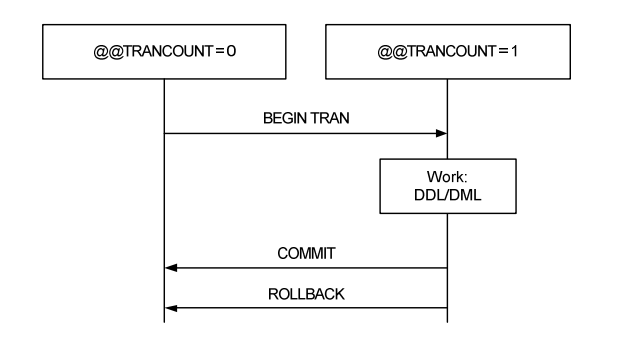
\includegraphics[width=0.4\textwidth]{img/t3.png}
	\end{center}
	\captionsetup{justification=centering}
\end{figure}


\subsection{Вложенные транзакции}

Когда явные транзакции вложены, т. е. расположены одна в другой, они называются вложенными транзакциями. Поведение инструкций COMMIT и
ROLLBACK изменяется для вложенных транзакций. 

\begin{figure}[h!]
	\begin{center}
		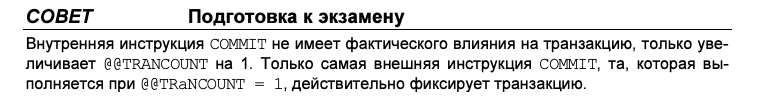
\includegraphics[width=0.8\textwidth]{img/advice25.png}
	\end{center}
	\captionsetup{justification=centering}
\end{figure}

\begin{figure}[h!]
	\begin{center}
		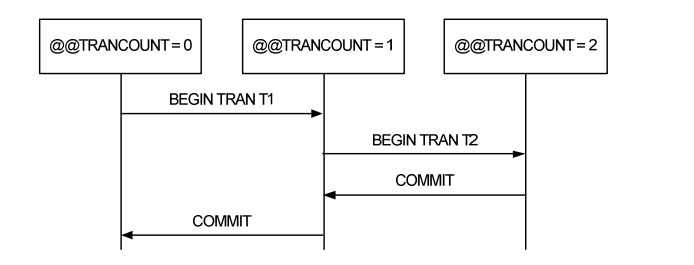
\includegraphics[width=0.8\textwidth]{img/t4.png}
	\end{center}
	\caption{Финальная самая внешняя инструкция COMMIT во вложенной транзакции}
	\captionsetup{justification=centering}
\end{figure}


\begin{figure}[h!]
	\begin{center}
		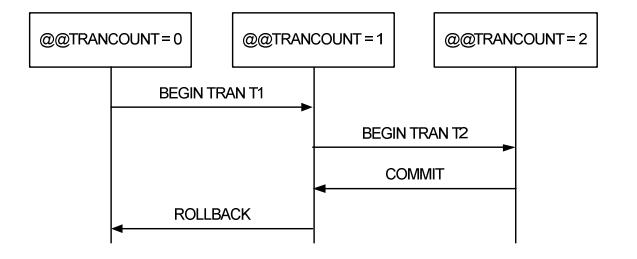
\includegraphics[width=0.8\textwidth]{img/t5.png}
	\end{center}
	\caption{Конечная инструкция ROLLBACK, выполняющая откат всей транзакции}
	\captionsetup{justification=centering}
\end{figure}

\begin{figure}[h!]
	\begin{center}
		
\includegraphics[width=0.8\textwidth]{img/advice26.png}
	\end{center}
	\captionsetup{justification=centering}
\end{figure}

\subsection{Разметка транзакции}

Именованные транзакции используются для помещения метки в журнал транзакций, чтобы указать точку, в которую могут быть восстановлены одна или более баз
данных.


\begin{lstlisting}[label=lst:funcReturn, language=sql]
	USE TSQL2012;
	BEGIN TRAN Tran1 WITH MARK;
	...
	COMMIT TRAN;
	...

	...
	RESTORE DATABASE TSQ2012 FROM DISK = 'C:\SQLBackups\TSQL2012.bak'
 	WITH NORECOVERY;

	RESTORE LOG TSQL2012 FROM DISK = 'C:\SQLBackups\TSQL2012.trn'
 	WITH STOPATMARK = 'Tran1';
\end{lstlisting}

При использовании предложения WITH MARK необходимо помнить следующее. 


\begin{itemize}
	\item Вы должны использовать имя транзакции с ключевым словом WITH STOPATMARK. 
	\item Вы можете поместить описание после предложения WITH MARK, но SQL Server
	будет его игнорировать. 
	\item Вы можете выполнить восстановление на момент непосредственно перед транзакцией с помощью предложения STOPBEFOREMARK. 
	\item Можно восстановить базу данных из копии с использованием ключевых слов
	WITH STOPATMARK или STOPBEFOREMARK. 
	\item Вы можете добавить параметр RECOVERY в списке WITH, но это не будет иметь
	никакого эффекта. 
\end{itemize}


\subsection{Дополнительные параметры транзакции}

\begin{itemize}
	\item \textbf{Точки сохранения}. Это точки внутри транзакций, которые можно использовать
	для отката выборочной части работы. Можно определить точку сохранения с помощью команды SAVE TRANSACTION.
	\item \textbf{Межбазовые транзакции}. Транзакция может охватывать одну или более баз
	данных на одном экземпляре SQL Server без каких-либо дополнительных действий на стороне пользователя. 
	\item \textbf{Распределенные транзакции}. Транзакция может распространяться на несколько серверов с помощью связанного сервера. Такая транзакция называется распределенной (в противоположность локальной) транзакцией. 
\end{itemize}

\begin{figure}[h!]
	\begin{center}
		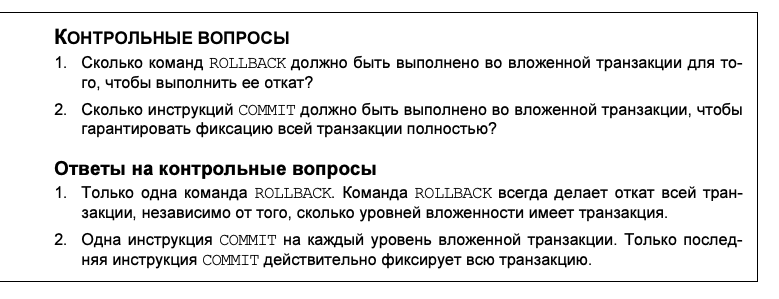
\includegraphics[width=0.8\textwidth]{img/control29.png}
	\end{center}
	\captionsetup{justification=centering}
\end{figure}


\subsection{Основные блокировки}

Чтобы сохранить изоляцию транзакций, SQL Server реализует набор протоколов
блокирования. На базовом уровне существуют два основных режима блокировок: 

\begin{itemize}
	\item совмещаемые блокировки (shared locks) используются для сеансов, выполняющих чтение данных, т. е. для операций считывания;
	\item монопольные блокировки (exclusive locks) используются для изменений данных,
	т. е. для операций записи. 
\end{itemize}

\begin{figure}[h!]
	\begin{center}
		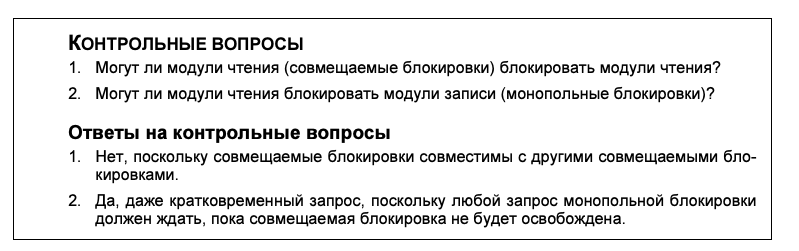
\includegraphics[width=0.8\textwidth]{img/control30.png}
	\end{center}
	\captionsetup{justification=centering}
\end{figure}


\begin{figure}[h!]
	\begin{center}
		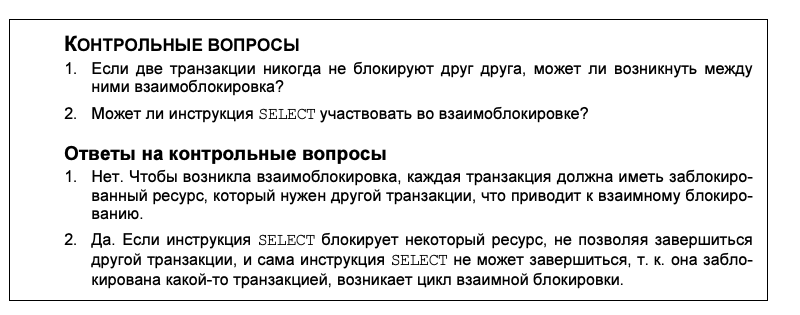
\includegraphics[width=0.8\textwidth]{img/control31.png}
	\end{center}
	\captionsetup{justification=centering}
\end{figure}

\subsection{Уровни изоляции транзакций}

К наиболее часто используемым уровням изоляции относятся следующие. 

\begin{itemize}
	\item \textbf{READ COMMITTED}. Это уровень изоляции по умолчанию. Все модули чтения в данном сеансе будут только выполнять чтение изменений данных, которые были
	зафиксированы. Поэтому все инструкции SELECT будут пытаться получить совмещаемые блокировки, и любые базовые ресурсы данных, которые изменяются
	в разных сеансах и, следовательно, имеют монопольные блокировки, будут блокировать сеанс READ COMMITTED. 
	\item \textbf{READ UNCOMMMITED}. Этот уровень изоляции позволяет модулям чтения читать незафиксированные данные. Эта настройка удаляет совмещаемые блокировки, полученные инструкциями SELECT, так что модули чтения больше уже не блокируются модулями записи. Но результаты инструкции SELECT могут считывать незафиксированные данные, которые были изменены в течение транзакции и
	позже откатывались к их первоначальному состоянию. Это называется "грязным" чтением данных. 
	\item \textbf{READ COMMITTED SNAPSHOT}. Фактически это не новый уровень изоляции; это дополнительный способ использования уровня изоляции по умолчанию READ
	COMMITTED, уровень изоляции по умолчанию в базе данных Windows Azure SQL.
\end{itemize}


Следующие уровни изоляции обеспечивают более строгий контроль над тем, какие данные могут быть прочитаны между
транзакциями. Поскольку они могут приводить к еще большему блокированию
или большим затратам, они не используются так часто, как более слабые уровни
изоляции. 


\begin{itemize}
	\item \textbf{REPEATABLE READ}. Этот уровень изоляции, также устанавливаемый на уровне сеанса, гарантирует, что данные, считанные в транзакции, могут быть позднее
	снова прочитаны в транзакции. Не допускаются операции обновления и удаления уже выбранных строк. В результате совмещаемые блокировки удерживаются до конца транзакции. Однако транзакция может видеть новые строки, добавленные после первой операции чтения; это называется фантомным чтением. 
	\item \textbf{SNAPSHOT}. Этот уровень изоляции также использует управление версиями строк
	в базе данных tempdb (как это делает RCSI). Он разрешен как постоянное свойство базы данных и поэтому устанавливается на отдельную транзакцию. Транзакция, использующая уровень изоляции SNAPSHOT, сможет повторить любую операцию чтения, и при этом она не будет видеть никаких фантомных чтений. Новые строки могут быть добавлены в таблицу, но транзакция не будет их видеть.
	Поскольку она использует управление версиями строк, уровень изоляции
	SNAPSHOT не требует совмещаемых блокировок на базовых данных. 
	\item \textbf{SERIALIZABLE}. Этот уровень изоляции является наиболее строгим и устанавливается на сеанс. На этом уровне все операции чтения являются повторяемыми,
	и новые строки не разрешены в базовых таблицах, что может удовлетворять условиям инструкций SELECT в транзакции. 
\end{itemize}


\begin{figure}[h!]
	\begin{center}
		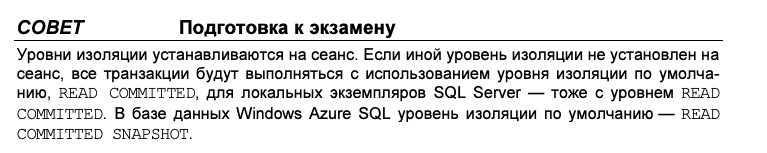
\includegraphics[width=0.8\textwidth]{img/advice27.png}
	\end{center}
	\captionsetup{justification=centering}
\end{figure}

\begin{figure}[h!]
	\begin{center}
		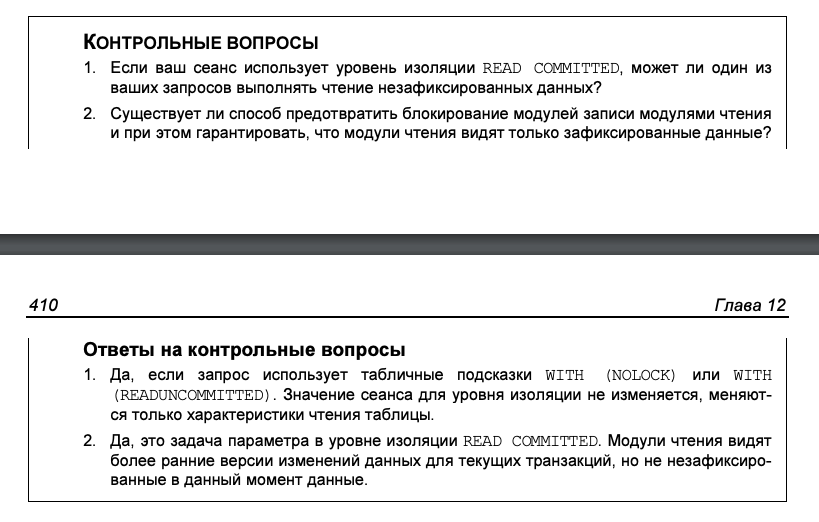
\includegraphics[width=0.8\textwidth]{img/control32.png}
	\end{center}
	\captionsetup{justification=centering}
\end{figure}


\subsection*{Резюме занятия}
\begin{itemize}
\item Все изменения данных в SQL Server происходят в контексте транзакции. Выполнение команды ROLLBACK на любом уровне вложенности транзакции немедленно откатывает всю транзакцию полностью. 
\item Каждая инструкция COMMIT уменьшает значение @@TRANCOUNT на 1, и только самая
внешняя инструкция COMMIT фиксирует всю вложенную транзакцию. 
\item SQL Server использует блокирование для обеспечения изоляции транзакций. 
\item Взаимоблокировка может возникнуть между двумя или более сеансами, если
каждый сеанс получил несовместимые блокировки, которые нужны другому
сеансу для завершения его инструкции. Когда SQL Server видит взаимоблокировку, он выбирает один из сеансов и прерывает пакет. 
\item SQL Server обеспечивает ACID-свойство, называемое уровнем изоляции, с разной степенью строгости. 
\item Уровень изоляции READ COMMITTED — это уровень изоляции по умолчанию для
локального SQL Server. 
\item Параметр изоляции READ COMMITTED SNAPSHOT (RCSI) уровня изоляции по умолчанию позволяет запросам на чтение получать доступ к ранее зафиксированным
версиям монопольно заблокированных данных. Это может значительно снизить
блокирование и взаимоблокирование. RCSI — это уровень изоляции по умолчанию в базе данных Windows Azure SQL. 
\item  Уровень изоляции READ UNCOMMITTED разрешает сеансу считывать незафиксированные данные, известные как "грязные чтения". 
\end{itemize}

\subsection*{Закрепление материала}

\begin{figure}[h!]
	\begin{center}
		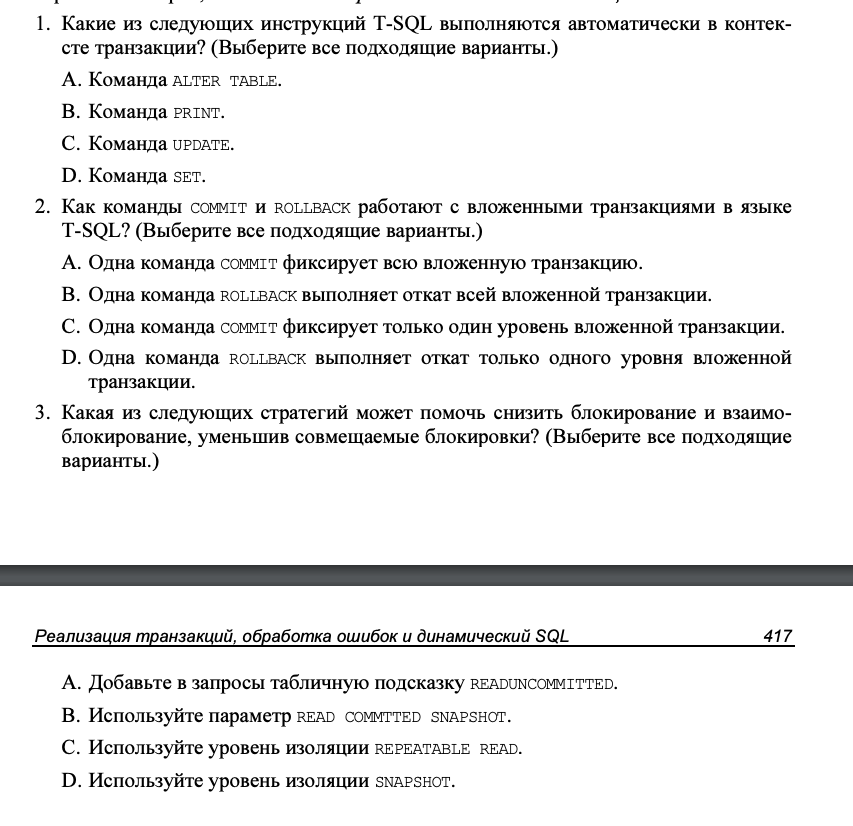
\includegraphics[width=0.7\textwidth]{img/zakrep23.png}
	\end{center}
	\captionsetup{justification=centering}
\end{figure}
\newpage

\subsection*{Ответы}

\begin{figure}[h!]
	\begin{center}
		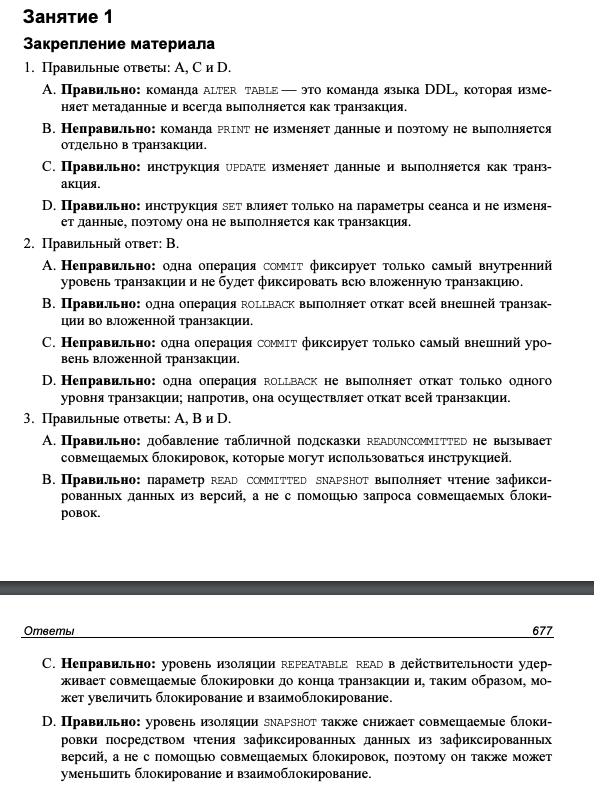
\includegraphics[width=0.9\textwidth]{img/ans27.png}
	\end{center}
	\captionsetup{justification=centering}
\end{figure}
\clearpage



\section{Реализация обработки ошибок}

\subsection{Анализ сообщений об ошибке }
Далее приведен пример сообщения об ошибке от SQL Server 2012. 

\begin{figure}[h!]
	\begin{center}
		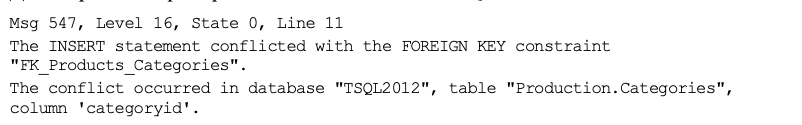
\includegraphics[width=0.9\textwidth]{img/error.png}
	\end{center}
	\captionsetup{justification=centering}
\end{figure}

Сообщения об ошибке в SQL Server состоит из четырех частей
\begin{itemize}
	\item \textbf{Номер ошибки} (error number) — это целочисленное значение. Нумеруются от 1 до 49 999. Пользовательские сообщения об ошибках нумеруются с 50 001 и выше.
	\item \textbf{Уровень серьезности}. В SQL Server определено 26 уровней серьезности с номерами от 0 до 25. По общему правилу, ошибки с уровнем серьезности от 16 и выше автоматически записываются в журнал SQL Server и в журнал приложений Windows. Ошибки с уровнем серьезности от 19 до 25 могут быть указаны только членами предопределенной роли сервера sysadmin. Ошибки с уровнем серьезности от 20 до 25 считаются фатальными (неустранимыми) и приводят к разрыву соединений и откату всех открытых транзакций. Ошибки с уровнем серьезности 0 до 10 являются информационными. 
	\item \textbf{Состояние (state)} --- целое число с максимальным значением 127, используемое
	компанией Microsoft для внутренних целей. 
	\item \textbf{Сообщение об ошибке} (error message) может иметь длину до 255 символов в кодировке Unicode. Сообщения об ошибках SQL Server перечислены в представлении каталога
	sys.messages. Можно добавлять пользовательские сообщения об ошибках с помощью процедуры sp\_addmessage. 
\end{itemize}

\subsection{Команда THROW}

Команда THROW во многом ведет себя так же, как команда RAISERROR, за некоторыми
важными исключениями. Базовый синтаксис команды THROW выглядит следующим
образом: 


\begin{lstlisting}[label=lst:funcReturn, language=sql]
	THROW [ { error_number | @local_variable },
	{ message | @local_variable },
	{ state | @local_variable }
	][; ]
\end{lstlisting}

Команда THROW имеет множество таких же компонентов, что и команда RAISERROR,
но со следующими значительными отличиями: 
\begin{itemize}
	\item команда THROW может использоваться без параметров, но только в блоке CATCH
	конструкции TRY/CATCH; 
	\item если имеются параметры, то номер ошибки, сообщение и состояние являются
	обязательными;
	\item номер ошибки error\_number не требует соответствующего сообщения, определенного в представлении каталога sys.messages; 
	\item параметр сообщения не допускает форматирование, но можно использовать
	функцию FORMATMESSAGE() с переменной для получения того же результата; 
	\item параметр состояния (state) должен быть целым числом в диапазоне от 0 до 255; 
	\item любой параметр может быть переменной;
	\item параметр серьезности ошибки не используется, уровень серьезности ошибки
	всегда устанавливается равным 16; 
	\item команда THROW всегда прерывает выполнение пакета, за исключением случаев,
	когда она используется в блоке TRY. 
\end{itemize}


\begin{figure}[h!]
	\begin{center}
		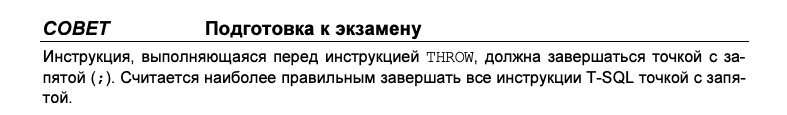
\includegraphics[width=0.9\textwidth]{img/advice30.png}
	\end{center}
	\captionsetup{justification=centering}
\end{figure}

В качестве примера можно вызвать простую инструкцию THROW следующим образом: 


\begin{lstlisting}[label=lst:funcReturn, language=sql]
	THROW 50000, 'Error in usp_InsertCategories stored procedure', 0; 
\end{lstlisting}

\subsection*{Функции TRY\_CONVERT и TRY\_PARSE}

Функция TRY\_CONVERT пытается
привести значение к выходному типу данных и в случае успеха возвращает это значение, в противном случае возвращается значение NULL. 

\begin{lstlisting}[label=lst:funcReturn, language=sql]
	SELECT TRY_CONVERT(DATETIME, '1752-12-31');
	SELECT TRY_CONVERT(DATETIME, '1753-01-01');
\end{lstlisting}

Функция TRY\_PARSE позволяет принимать входную строку, содержащую данные
с неопределенным типом данных и преобразовывать их в конкретный тип данных
при возможности, или возвращать NULL в противном случае. В следующем примере
выполняет синтаксический анализ двух строк. 

\begin{lstlisting}[label=lst:funcReturn, language=sql]
	SELECT TRY_PARSE('1' AS INTEGER);
	SELECT TRY_PARSE('B' AS INTEGER); 
\end{lstlisting}

\begin{figure}[h!]
	\begin{center}
		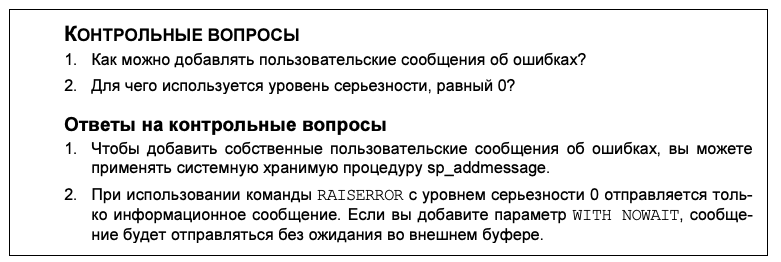
\includegraphics[width=0.9\textwidth]{img/control33.png}
	\end{center}
	\captionsetup{justification=centering}
\end{figure}

\subsection{Неструктурированная обработка ошибок с помощью функции @@ERROR}

Неструктурированная обработка ошибок заключается в проверке отдельных инструкций на их состояние ошибки непосредственно после их выполнения. Для этого
необходимо запросить системную функцию @@ERROR.
Основная проблема неструктурированной обработки ошибок — необходимость
проверять @@ERROR после каждой модификации данных или инструкции DML. Поскольку центральное местоположение для обработки ошибок не предоставляется,
обработка ошибок должна выполняться в пользовательском коде. 

\subsection{Использование параметра XACT\_ABORT с транзакциями}


Поставив в начало пакета SET XACT\_ABORT ON, можно вызвать сбой всего этого
пакета в случае возникновения ошибки. XACT\_ABORT устанавливается на отдельный
сеанс.

\subsection{Структурированная обработка ошибок с помощью конструкции TRY/CATCH}

Далее приведены некоторые правила использования конструкции TRY/CATCH

\begin{itemize}
	\item Ошибки с уровнем серьезности больше 10 и меньше 20 в блоке TRY приводят
	к передаче управления блоку CATCH. 
	\item Ошибки с уровнем серьезности больше 10 и меньше 20 в блоке TRY приводят
	к передаче управления блоку CATCH. 
	\item Ошибки компиляции и некоторые ошибки выполнения программы, задействующие компиляцию уровня инструкции, прерывают выполнение пакета немедленно и не передают управление CATCH. 
	\item Если ошибка произошла в блоке CATCH, транзакция прерывается и ошибка возвращается вызывающему приложению, если блок CATCH не вложен в блок TRY. 
	\item В блоке CATCH можно выполнить фиксацию или откат текущей транзакции, если транзакция не может быть зафиксирована и ее необходимо откатить. Для проверки состояния транзакции можно запросить функцию XACT\_STATE. 
	\item Блок TRY/CATCH не перехватывает ошибки, приводящие к прерыванию соединения, такие как неустранимая ошибка или выполнение ролью sysadmin команды KILL. 
	\item Также невозможно перехватить ошибки, которые возникают из-за ошибок компиляции, синтаксических ошибок или несуществующих объектов. Поэтому вы не можете использовать конструкцию TRY/CATCH для проверки существования объекта.
	\item Блоки TRY/CATCH могут быть вложенными; другими словами, можно поместить внутренний блок TRY/CATCH во внешний блок TRY. Ошибка внутри вложенного блока TRY передает выполнение соответствующему вложенному блоку CATCH. 
\end{itemize}

\begin{lstlisting}[label=lst:funcReturn, language=sql]
	BEGIN CATCH
	 SELECT ERROR_NUMBER() AS errornumber
	 , ERROR_MESSAGE() AS errormessage
	 , ERROR_LINE() AS errorline
	 , ERROR_SEVERITY() AS errorseverity
	 , ERROR_STATE() AS errorstate;
	END CATCH; 
\end{lstlisting}

\begin{figure}[h!]
	\begin{center}
		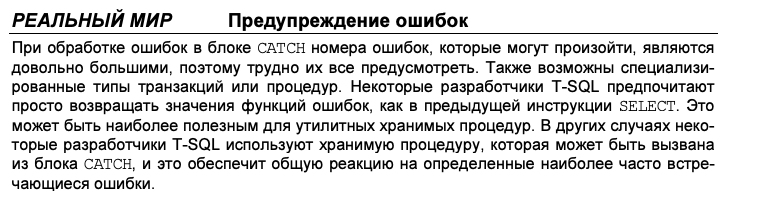
\includegraphics[width=0.9\textwidth]{img/advice34.png}
	\end{center}
	\captionsetup{justification=centering}
\end{figure}

\begin{figure}[h!]
	\begin{center}
		
\includegraphics[width=0.9\textwidth]{img/advice35.png}
	\end{center}
	\captionsetup{justification=centering}
\end{figure}

\begin{figure}[h!]
	\begin{center}
		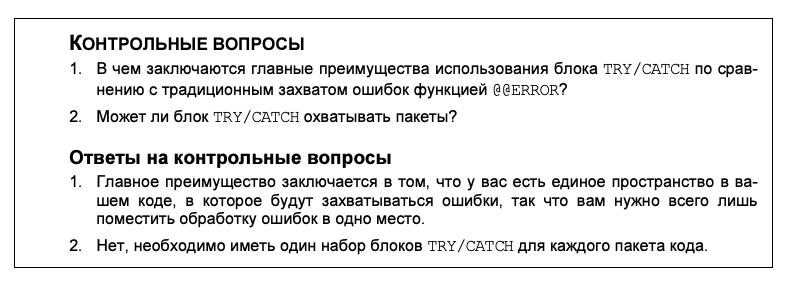
\includegraphics[width=0.9\textwidth]{img/control34.png}
	\end{center}
	\captionsetup{justification=centering}
\end{figure}

		
\subsection*{Резюме занятия}
\begin{itemize}
\item SQL Server 2012 использует команды RAISERROR и THROW для генерации ошибок. 
\item Можно запросить системную функцию @@ERROR для определения, произошла ли ошибка и какой у нее номер. 
\item Можно использовать команду SET XACT\_ABORT ON, чтобы вызвать сбой транзакции и прерывание пакета, когда возникнет ошибка. 
\item Неструктурированная обработка ошибок не предоставляет единого места в коде для обработки ошибок. 
\item Блок TRY/CATCH предоставляет каждому блоку кода T-SQL блок CATCH, в котором выполняется обработка ошибок. 
\item Команда THROW может быть использована для повторной выдачи ошибок. 
\item Существует полный набор функций обработки ошибок для сбора информации об ошибках. 
\end{itemize}

\subsection*{Закрепление материала}

\begin{figure}[h!]
	\begin{center}
		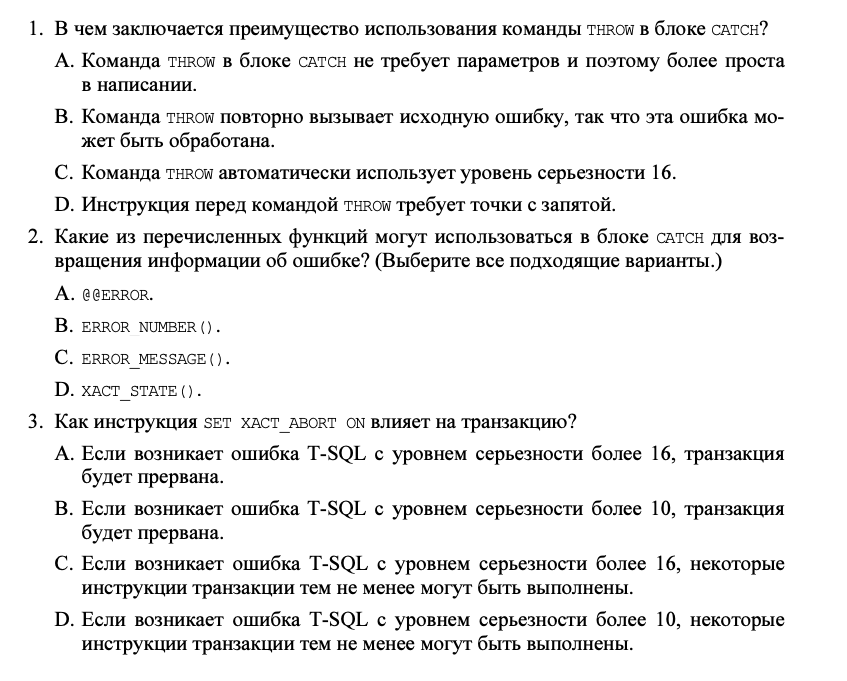
\includegraphics[width=0.9\textwidth]{img/zakrep27.png}
	\end{center}
	\captionsetup{justification=centering}
\end{figure}
\clearpage

\subsection*{Ответы}

\begin{figure}[h!]
	\begin{center}
		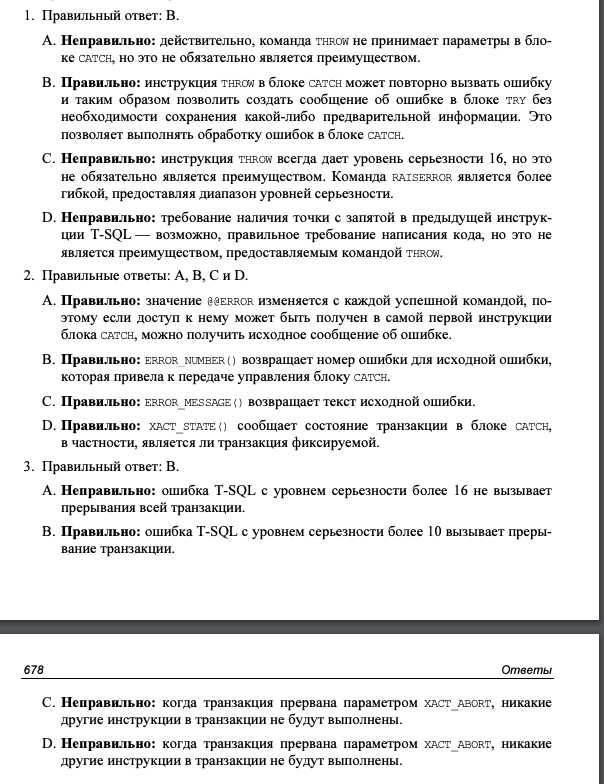
\includegraphics[width=0.9\textwidth]{img/ans28.png}
	\end{center}
	\captionsetup{justification=centering}
\end{figure}



\section{Использование динамического SQL}


Динамический SQL является полезной возможностью, т. к. T-SQL не разрешит
прямую замену многих частей команд переменными, включая следующие: 

\begin{itemize}
	\item имя базы данных в инструкции USE; 
	\item имена таблиц в предложении FROM; 
	\item  имена столбцов в предложениях SELECT, WHERE, GROUP BY и HAVING, а также в предложении ORDER BY; 
	\item содержимое списков, например, в предложениях IN и PIVOT. 
	\item Генерация кода для автоматизации административных задач. 
	\item Выполнение итераций во всех базах данных на сервере, во всех типах объектов
	в базе данных и в метаданных объектов, таких как имена столбцов или индексы. 
	\item Построение хранимых процедур с множеством необязательных параметров, составляющих результирующие запросы, на основании которых параметры получают значения.
\end{itemize}


\subsection{Инструкция EXECUTE}
Простейший способ, предоставляемый SQL Server для выполнения динамического
SQL, — это инструкция EXECUTE, которую можно записывать как EXECUTE или сокращенно EXEC.

Далее перечислены особенности использования команды EXEC, которые следует знать.

\begin{itemize}
	\item Входная строка должна быть одним пакетом T-SQL. Строка может содержать
	множество команд T-SQL, но она не может содержать разделители GO. 
	\item Можно использовать строковые литералы, строковые переменные или их объединение. 
\end{itemize}


\begin{lstlisting}[label=lst:funcReturn, language=sql]
	DECLARE @SQLString AS NVARCHAR(MAX)
	, @tablename AS NVARCHAR(261) = '[Production].[Products]';
   	SET @SQLString = 'SELECT COUNT(*) AS TableRowCount FROM '
   	EXEC(@SQLString + @tablename);
\end{lstlisting}


\begin{figure}[h!]
	\begin{center}
		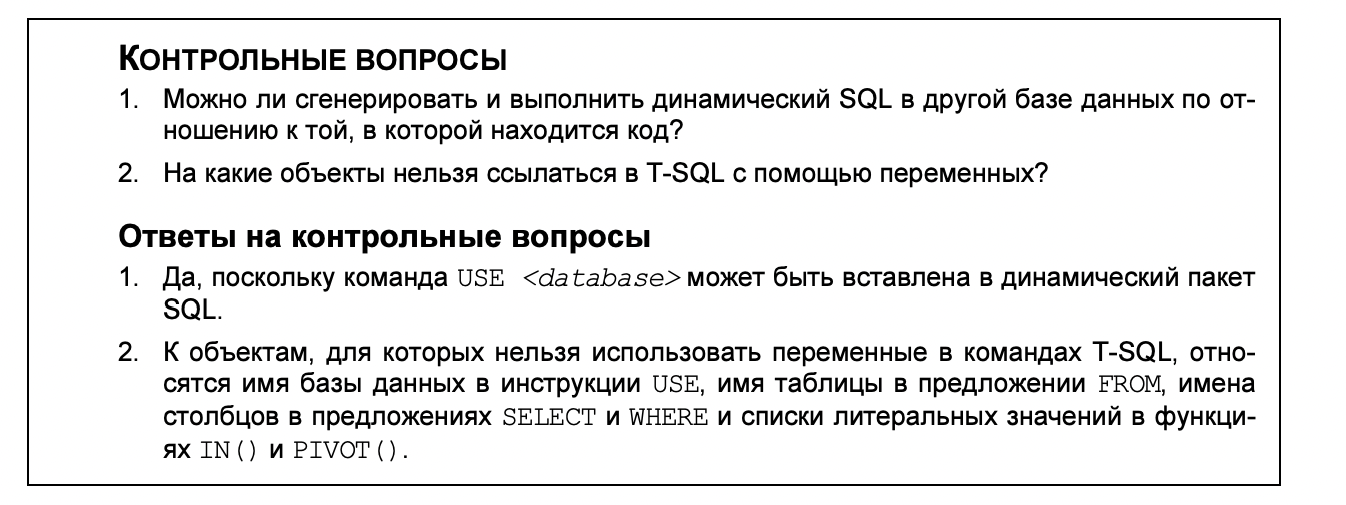
\includegraphics[width=0.9\textwidth]{img/control35.png}
	\end{center}
	\captionsetup{justification=centering}
\end{figure}


\begin{figure}[h!]
	\begin{center}
		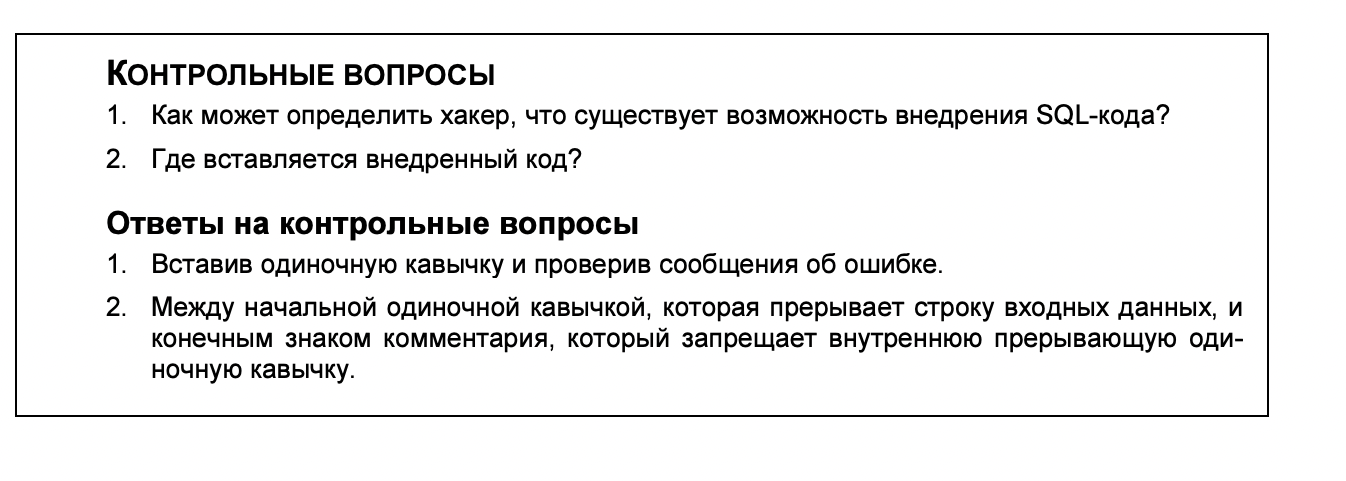
\includegraphics[width=0.9\textwidth]{img/control36.png}
	\end{center}
	\captionsetup{justification=centering}
\end{figure}


\subsection{Использование хранимой процедуры sp\_executesql}


Поддерживаются выходные параметры. Благодаря параметрам, системная хранимая процедура sp\_executesql является более безопасной и может помочь предотвратить некоторые виды внедрения SQL-кода. Параметры sp\_executesql не могут быть
использованы для замещения необходимых строковых литералов, таких как имена
таблиц и столбцов. 


\begin{lstlisting}[label=lst:funcReturn, language=sql]
	sp_executesql [ @statement = ] statement
	[ {, [ @params = ] N'@parameter_name data_type [ OUT | OUTPUT ][,...n ]' }
	 {, [ @param1 = ] 'value1' [ ,...n ] }] 
\end{lstlisting}

Входной параметр @statement имеет тип данных NVARCHAR(MAX). Вам нужно представить инструкцию в виде Unicode-строки в параметр @statement и встроить в эту
инструкцию параметры, которые должны быть заменены в финальной строке. Вы
должны перечислить имена этих параметров вместе с их типами данных в строке
@params, а затем поместить значения в списки @param1, @param2 и т. д. 


\begin{figure}[h!]
	\begin{center}
		
\includegraphics[width=0.9\textwidth]{img/advice31.png}
	\end{center}
	\captionsetup{justification=centering}
\end{figure}


Хранимая процедура sp\_executesql иногда обеспечивает лучшую производительность запроса, чем команда EXEC, т. к. параметризация способствует повторенному использованию кэшированных планов выполнения. Поскольку хранимая процедура
sp\_executesql принуждает к параметризации, часто строка запроса остается той же
самой, а изменяются только значения параметров.


\begin{figure}[h!]
	\begin{center}
		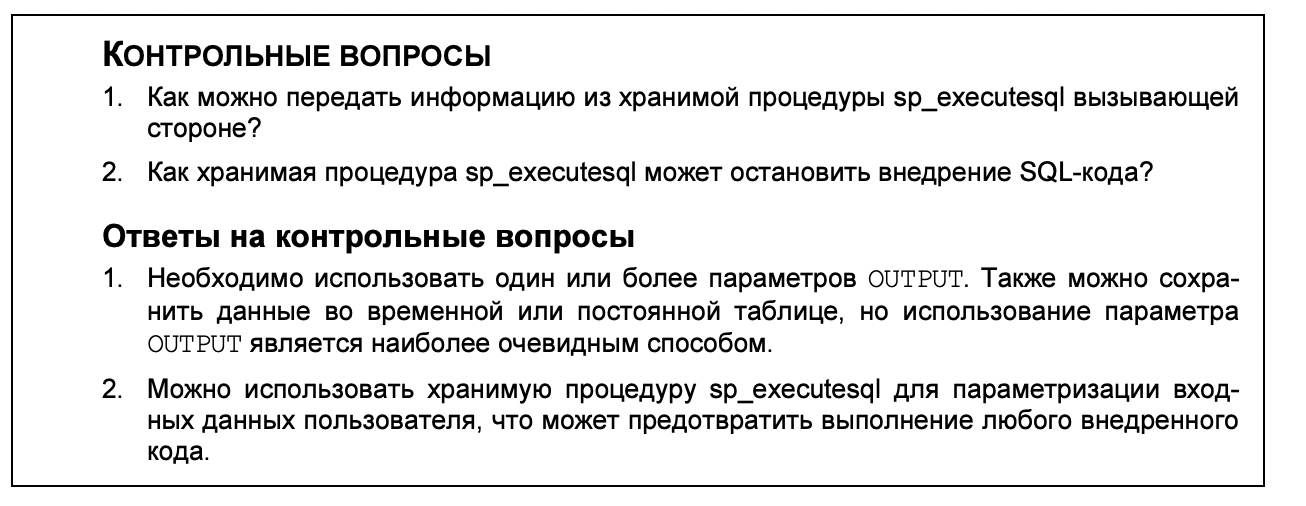
\includegraphics[width=0.9\textwidth]{img/control37.png}
	\end{center}
	\captionsetup{justification=centering}
\end{figure}



\subsection*{Резюме занятия}
\begin{itemize}
\item Динамический SQL можно использовать для генерации и выполнения кода
T-SQL в случаях, когда инструкции T-SQL должны строиться во время выполнения.
\item Внедрение SQL-кода означает потенциальную возможность для приложений
принимать входные данные, которые внедряют нежелательный код, выполняемый динамическим SQL. 
\item Хранимая процедура sp\_executesql может использоваться, чтобы помочь предотвратить внедрение SQL-кода, путем параметризации соответствующих частей
динамического SQL. 
\end{itemize}


\subsection*{Закрепление материала}

\begin{figure}[h!]
	\begin{center}
		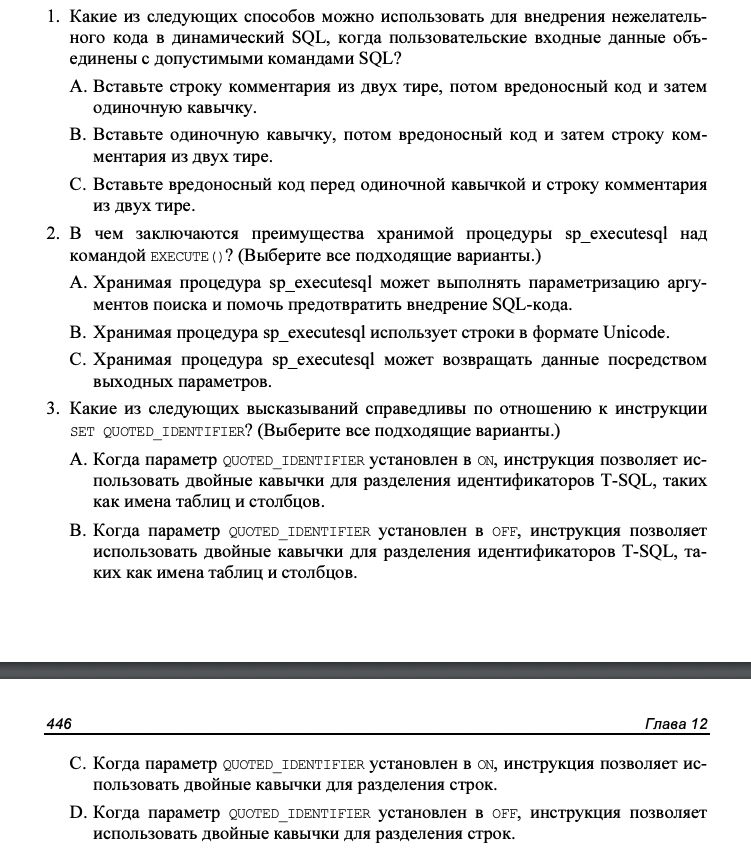
\includegraphics[width=0.7\textwidth]{img/zakrep28.png}
	\end{center}
	\captionsetup{justification=centering}
\end{figure}
\clearpage

\subsection*{Ответы}

\begin{figure}[h!]
	\begin{center}
		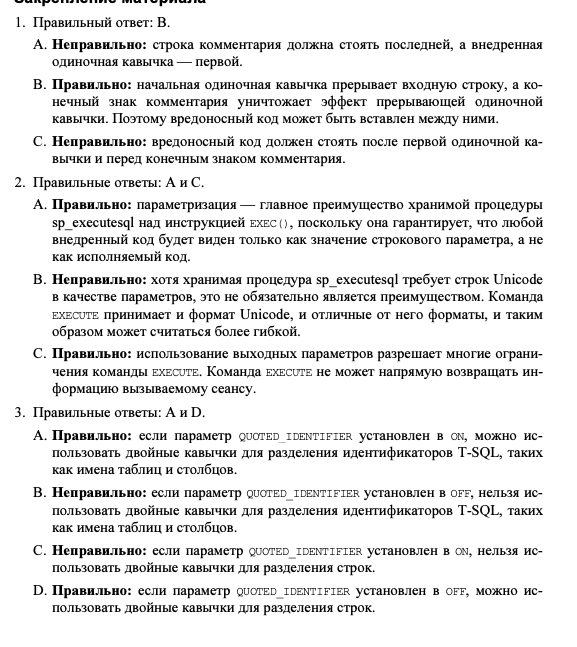
\includegraphics[width=0.9\textwidth]{img/ans29.png}
	\end{center}
	\captionsetup{justification=centering}
\end{figure}


\newpage
\subsection*{Упражнения}

\begin{figure}[h!]
	\begin{center}
		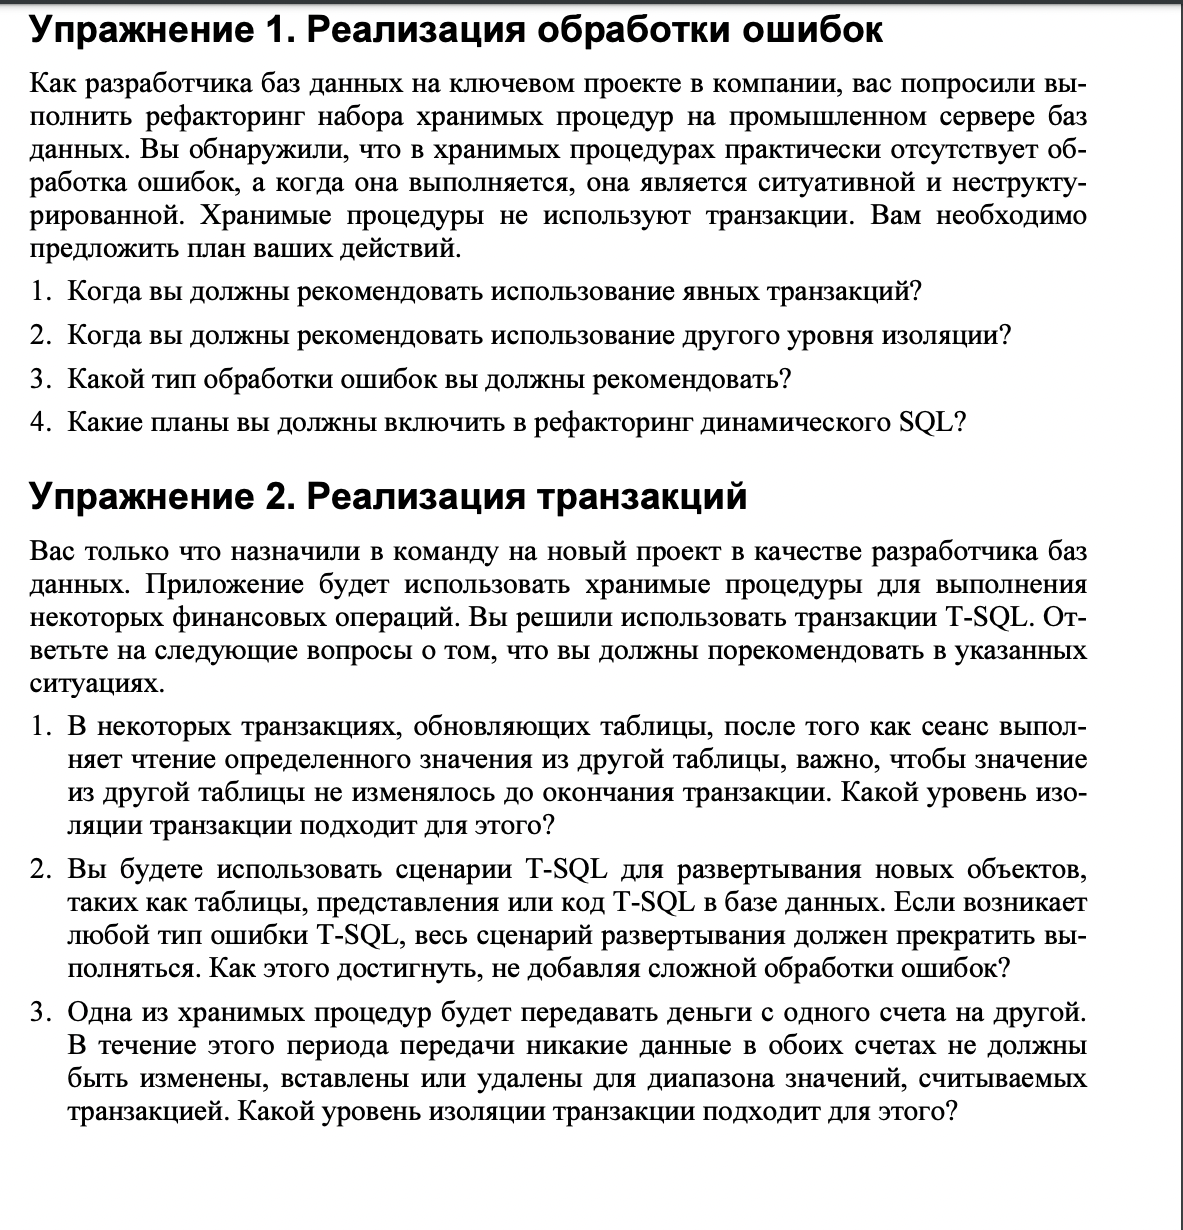
\includegraphics[width=0.9\textwidth]{img/ex21.png}
	\end{center}
	\captionsetup{justification=centering}
\end{figure}

\subsection*{Ответы}

\begin{figure}[h!]
	\begin{center}
		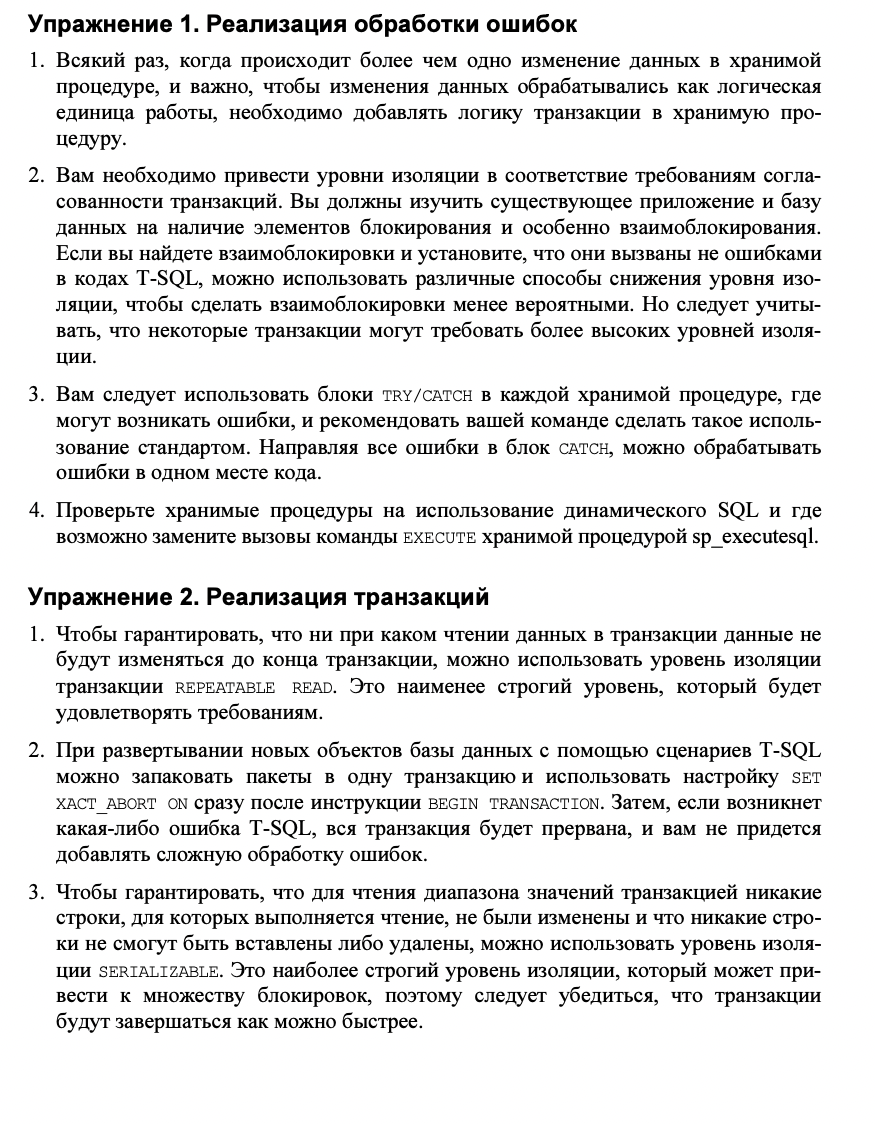
\includegraphics[width=0.9\textwidth]{img/eans21.png}
	\end{center}
	\captionsetup{justification=centering}
\end{figure}